%%%%%%%%%%%%%%%%%%%%%%%%%%%%%%%%%%%%%%%%%%%%%%%%%%%%%%%%%%%%%%%%%%%%%%%%%%%%%%%%
%%%%%%%%%%%%%%%%%%%%%%%%%%%%%%%%%%%%%%%%%%%%%%%%%%%%%%%%%%%%%%%%%%%%%%%%%%%%%%%%
%%% Template for AIMS Rwanda Assignments         %%%              %%%
%%% Author:   AIMS Rwanda tutors                             %%%   ###        %%%
%%% Email: tutors2017-18@aims.ac.rw                               %%%   ###        %%%
%%% Copyright: This template was designed to be used for    %%% #######      %%%
%%% the assignments at AIMS Rwanda during the academic year %%%   ###        %%%
%%% 2017-2018.                                              %%%   #########  %%%
%%% You are free to alter any part of this document for     %%%   ###   ###  %%%
%%% yourself and for distribution.                          %%%   ###   ###  %%%
%%%                                                         %%%              %%%
%%%%%%%%%%%%%%%%%%%%%%%%%%%%%%%%%%%%%%%%%%%%%%%%%%%%%%%%%%%%%%%%%%%%%%%%%%%%%%%%
%%%%%%%%%%%%%%%%%%%%%%%%%%%%%%%%%%%%%%%%%%%%%%%%%%%%%%%%%%%%%%%%%%%%%%%%%%%%%%%%


%%%%%% Ensure that you do not write the questions before each of the solutions because it is not necessary. %%%%%% 

\documentclass[12pt,a4paper]{article}

%%%%%%%%%%%%%%%%%%%%%%%%% packages %%%%%%%%%%%%%%%%%%%%%%%%
\usepackage{amsmath}
\usepackage{amssymb}
\usepackage{amsthm}
\usepackage{amsfonts}
\usepackage{graphicx}
\usepackage[all]{xy}
\usepackage{tikz}
\usepackage{verbatim}
\usepackage{float}
\usepackage[left=2cm,right=2cm,top=3cm,bottom=2.5cm]{geometry}
\usepackage{hyperref}
\usepackage{caption}
\usepackage{subcaption}
\usepackage{psfrag}
\usepackage{mathrsfs}

%%%%%%%%%%%%%%%%%%%%% students data %%%%%%%%%%%%%%%%%%%%%%%%
\newcommand{\student}{Yuusf Brima}
\newcommand{\course}{Statistical Machine Learning for Data Science}
\newcommand{\assignment}{1}

%%%%%%%%%%%%%%%%%%% using theorem style %%%%%%%%%%%%%%%%%%%%
\newtheorem{thm}{Theorem}
\newtheorem{lem}[thm]{Lemma}
\newtheorem{defn}[thm]{Definition}
\newtheorem{exa}[thm]{Example}
\newtheorem{rem}[thm]{Remark}
\newtheorem{coro}[thm]{Corollary}
\newtheorem{quest}{Question}[section]

%%%%%%%%%%%%%%  Shortcut for usual set of numbers  %%%%%%%%%%%

\newcommand{\N}{\mathbb{N}}
\newcommand{\Z}{\mathbb{Z}}
\newcommand{\Q}{\mathbb{Q}}
\newcommand{\R}{\mathbb{R}}
\newcommand{\C}{\mathbb{C}}

%%%%%%%%%%%%%%%%%%%%%%%%%%%%%%%%%%%%%%%%%%%%%%%%%%%%%%%555
\begin{document}

%%%%%%%%%%%%%%%%%%%%%%% title page %%%%%%%%%%%%%%%%%%%%%%%%%%
\thispagestyle{empty}
%\begin{figure}
%    \centering
%    \includegraphics[width=\textwidth]{aims_rwanda.jpg}
%\end{figure}
\begin{center}
\textbf{AFRICAN INSTITUTE FOR MATHEMATICAL SCIENCES \\[0.5cm]
(AIMS RWANDA, KIGALI)}
\vspace{1.0cm}
\end{center}

%%%%%%%%%%%%%%%%%%%%% assignment information %%%%%%%%%%%%%%%%
\noindent
\rule{17cm}{0.2cm}\\[0.3cm]
Name: \student \hfill Assignment Number: \assignment\\[0.1cm]
Course: \course \hfill Date: \today\\
\rule{17cm}{0.05cm}
\vspace{1.0cm}
\section*{Exercise 1}
Let  $D_n={(\mathrm{x}_i,yi) \overset{\text{iid}}{\sim} p_{\mathrm{x},y}(\mathrm{x},y) ,  \mathrm{x}_i \in \mathbb{R}, y_i \in \mathbb{R},   i= 1, ... , n}.$ Consider using the data $\mathscr{D}_n,$ to build mappings  $f: \mathrm{x} \to Y$,  such that $f\in \mathscr{H},$ where
\begin{equation}
	\mathscr{H} := \left\lbrace  \mathrm{x}  \to f(\mathrm{x}) =  \theta \mathrm{x} , \vspace{0.4pt}  \theta \in \mathbb{R}^{\text{*}} \right\rbrace
	\label{eq:1}
\end{equation}
We suppose that $\forall i \in [n]$, we have 
\begin{equation}
		\mathrm{p}(y_i|\mathrm{x}_i, \theta, \sigma^2) = \frac{1}{\sqrt{2 \pi \sigma^2  }} e^{ \frac{-1}{ 2\sigma^2} (y_i - f(\mathrm{x}_i))^2 }
		\label{eq:2}
\end{equation}
where $f \in \mathscr{H} $.  We let \textbf{x} $ = (\mathrm{x_1}, \mathrm{x_2},\mathrm{x_3}, ..., \mathrm{x_n})^{\text{T}} $ and \textbf{y} $ = (y_1, y_2, y_3,  ... , y_n)^{\text{T}} $ and define 
\begin{equation}
	\textbf{SSE}_n(a) =  \sum_{i =1}^{n} (y_i - a \mathrm{x}_i)^2 =   (\textbf{y} - a\textbf{x})    (\textbf{y} - a\textbf{x}) ^ {\text{T}} = || \textbf{y} - a\textbf{x} ||_2^2.  
	\label{eq:3}
\end{equation}
\begin{enumerate}
	\item[(1)] The input space in this problem,  and  its dimensionality is thus: $\mathscr{X} \in \mathbb{R}$  and dim($\mathscr{X} $) = 1
	\item[(2)] The output space in this problem,  and  its dimensionality is thus: $\mathscr{Y} \in \mathbb{R}$  and dim($\mathscr{Y} $) = 1
	\item[(3)]  The dimensionality of \textbf{x} is $\mathbb{R}^{n \times 1}$ 
	\item[(4)]  The dimensionality of \textbf{y} is $\mathbb{R}^{n \times 1}$ 
	\item[(5)] The assumed conditional distribution of $\textbf{y}_i$ given $\mathrm{x}_i$ and deduce the distribution \textbf{y} given \textbf{x}  is thus:
	\begin{align*}
				\mathrm{p}(y_i | \mathrm{x}_i) &= \phi(y_i, f(\mathrm{x}_i), \sigma^2)
	\end{align*}
	where
		\begin{align*}
				y_i =  f(\mathrm{x}_i + \epsilon_i)\\
				    &=  \mathrm{x}_i \theta + \epsilon_i\\
				    &= \mathrm{x}_i \theta
		\end{align*}
	\begin{align*}
			\mathrm{p}(y_i | \mathrm{x}_i) &=  \frac{1}{\sqrt{2 \pi \sigma^2  }} e^{ \frac{-1}{ 2\sigma^2} (y_i - f(\mathrm{x}_i))^2 }\\
					&=  \frac{1}{\sqrt{2 \pi \sigma^2  }} e^{ \frac{-1}{ 2\sigma^2} (y_i - \mathrm{x}_i \theta )^2 }\\
					&=  \eta(f(\mathrm{x}_i),\sigma^2) \\
					&= \eta(\mathrm{x}_i \theta, \sigma^2)
	\end{align*}
	
	\item[(6)] Rewriting the model defined by Equation \eqref{eq:2}  in its additive form featuring the deterministic component (signal) and the stochastic component (noise or error term). Be sure to reflect the fact that $f \in  \mathscr{H} $ as defined in Equation \eqref{eq:1}
	\begin{align*}
			y_i  &=  f(\mathrm{x}_i) + \epsilon_i \quad \text{where } \epsilon_i \overset{\text{iid}} \sim \mathcal{N}(0, \sigma^2)\\
		\underbrace{y_i}_{\text{observation}}  &=  \underbrace{ \mathrm{x}_i\theta }_{\text{deterministic signal}} + \underbrace{ \epsilon_i }_{stochastic noise}  \quad \text{and }  f \in  \mathscr{H}
	\end{align*}
	\item[(7)]  Type Statistical Machine Learning task is being solved  is Simple Linear Regression (SLR) and the justification is $\mathrm{x}_i \in \mathbb{R}$ which is a single predictor variable and $y_i \in \mathbb{R}$ which is continuous.
	\item[(8)] Using the appropriate tools to find $\frac{\partial\textbf{SSE}_n(a)}{\partial_a} $
	\begin{align*}
			\frac{\partial\textbf{SSE}_n(a)}{\partial_a} &=  \sum_{i=1}^n (y_i - \mathrm{x}_i a)^2  =  (y_i - \mathrm{x}_i a)    (y_i - \mathrm{x}_i a) ^ {\text{T}} = || y_i  - \mathrm{x}_i a ||_2^2.\\
			&=  \frac{\partial}{\partial a} (\sum_{i=1}^n (y_i -  \mathrm{x}_{ia} )^2  )\\
			&= -\sum_{i=1}^n 2\mathrm{x}_i (y_i - \mathrm{x}_{ia}) \\
			&= -2 ( \sum_{i=1}^n \mathrm{x}_i y_i  - a \sum_{i =1}^ n \mathrm{x}_i^2 )\\
			&=  -2(\mathrm{x}^{\text{T} }y - a \mathrm{x}^{\text{T} }\mathrm{x} ) 
	\end{align*}
	\item[(9)] Show that  
			\begin{align*}
					\hat{\theta} &=   \underset{\theta \in \mathbb{R}^ {*} } {\mathbf{argmin} \lbrace \textbf{SSE}_n(\theta ) }  \rbrace  =  \frac{\mathrm{x} ^{\text{T} }   \mathrm{y}} { \mathrm{x} ^{\text{T}} \mathrm{x} }
			\end{align*}
			\begin{align*}
					\frac{\partial\textbf{SSE}_n(a)}{\partial_a} &= 0  \iff  2(\mathrm{x}^{\text{T} } - a \mathrm{x}^{\text{T} }\mathrm{x} )  = 0\\
					a \mathrm{x}^{\text{T} }\mathrm{x}  &=  \mathrm{x}^{\text{T} }\mathrm{y}\\
						a &= \frac{\mathrm{x}^{\text{T} }\mathrm{y}}{\mathrm{x}^{\text{T} }\mathrm{x}  }
			\end{align*}
		\begin{align*}
				 \underset{\theta \in \mathbb{R}^ {*} } {\mathbf{argmin} \lbrace \textbf{SSE}_n(\theta ) }  = \frac{\mathrm{x}^{\text{T} }\mathrm{y}}{\mathrm{x}^{\text{T} }\mathrm{x}  }  = (\mathrm{x}^{\text{T} }\mathrm{x})^{-1} \mathrm{x}^{\text{T} }\mathrm{y}
		\end{align*}
		\item[(10)] Proving that mean$[\hat{\theta} ]$ = $\mathbb{E}[\hat{\theta}]$.
				\begin{align*}
						\mathbb{E}[\hat{\theta}] &=  \mathbb{E}[ (\mathrm{x}^{\text{T} }\mathrm{x})^{-1} \mathrm{x}^{\text{T} }\mathrm{y}] \\
						&=  (\mathrm{x}^{\text{T} }\mathrm{x})^{-1} \mathrm{x}^{\text{T} }\mathrm{y}\\ 
				\end{align*}
	But 
	\begin{align*}
			\mathrm{y} = \theta\mathrm{x} + \epsilon
	\end{align*}
Therefore 
		\begin{align*}
				\mathbb{E}[\hat{\theta}] &=   \theta \underbrace{ (\mathrm{x}^{\text{T} }\mathrm{x})^{-1} ((\mathrm{x}^{\text{T} }\mathrm{x}) )  }_{\text{identity matrix} } + \underbrace{ (\mathrm{x}^{\text{T} }\mathrm{x})^{-1}  \mathrm{x}^{\text{T}} \mathbb{E}[\epsilon] }_{0}\\
				&=  \theta \quad \text{so,  } \hat{\theta} \text{ is an unbiased estimator} 
		\end{align*}
		\item[(11)] Proving that variance$[\hat{\theta}] =  \mathbb{V}[\hat{\theta}]$  
				\begin{align*}
						 \mathbb{V}[\hat{\theta}] &=  \mathbb{V}[ \theta  (\mathrm{x}^{\text{T} }\mathrm{x})^{-1} \mathrm{x}^{\text{T} }\mathrm{x} +   (\mathrm{x}^{\text{T} }\mathrm{x})^{-1}  \mathrm{x}^{\text{T} }\epsilon  ]\\
						 &=   \mathbb{V}[ \theta +   (\mathrm{x}^{\text{T} }\mathrm{x})^{-1}  \mathrm{x}^{\text{T} }\epsilon  ]\\
						&=  \mathbb{V}[  (\mathrm{x}^{\text{T} }\mathrm{x})^{-1}  \mathrm{x}^{\text{T} }\epsilon  ]\\
							&=   ( (\mathrm{x}^{\text{T} }\mathrm{x})^{-1}  \mathrm{x}^{\text{T} })^{\text{T} } \mathbb{\epsilon }  (\mathrm{x}^{\text{T} }\mathrm{x})^{-1}  \mathrm{x}^{\text{T} }\\
							&=  (\mathrm{x}^{\text{T} }\mathrm{x})^{-1}  \sigma^2 \mathcal{I}_n  (\mathrm{x}^{\text{T} }\mathrm{x})^{-1}  \mathrm{x}^{\text{T} }\\
							&=  \sigma^2 (\mathrm{x}^{\text{T} }\mathrm{x})^{-1}
				\end{align*}
		\item[(12)] Finding the mean$(y_i|\mathrm{x}_i)  = \mathbb{E}[\mathrm{x}_i] \quad  \forall i \in [n]$ and deduce mean$(y|\mathrm{x}) =\mathbb{E}|x]$
		\begin{align*}
				\mathbb{E}[y_i | \mathrm{x}_i] &=  \mathbb{E}[\theta  \mathrm{x}_i  + \epsilon_i]  \\
				&= f(\mathrm{x}_i)\\
					&=  \theta   \mathbb{E}[ \mathrm{x}_i] ,  \quad  \mathrm{x}_i \in \mathbb{R} \text{ and}\\
					 &=  \theta \mathrm{x}_i ,  \quad \forall i \in [n] \quad \epsilon_i  \sim \mathcal{N}(0,\sigma^2)
		\end{align*}
			\begin{align*}
					\mathbb{E}[y|\mathrm{x}] &=  f(\mathrm{x}) \\
					&=  \theta \mathrm{x} , \quad \mathrm{x} \in \mathbb{R}^{n \times 1},  \theta \in \mathbb{R}
			\end{align*}					
		
		\item[(13)] To write down $y$ as a function of $\mathrm{x}  \theta$ and all other necessary parts of the assumed model in keeping with Equation \eqref{eq:2} is as follows: 
	\begin{align*}
			y &=   f(\mathrm{x}) +  \epsilon \quad \text{ where }  \epsilon  \sim \mathcal{N}(0,\sigma^2 \mathcal{I}_n)\\
				 &=  \theta \mathrm{x} + \epsilon \quad \mathrm{x} \in \mathbb{R}^{n \times 1}\\
				 \text{ and } \mathrm{p}(y,\mathrm{x},\sigma^2)  &=  \underset{\text{=}}{1}e^{\frac{-((y -  \theta \mathrm{x})^2 }{ 2\sigma^2}}
	\end{align*}
		
		\item[(14)] To write  $\hat{y}$ as  function of $\mathrm{x}$ and $y$ is as follows:
				\begin{align*}
						\hat{y} &=  \mathrm{x} \hat{\theta} \\
									&=  \mathrm{x}\lbrace (\mathrm{x}^{\text{T} } \mathrm{x})^{-1} \mathrm{x}^{\text{T} } y   \rbrace 
				\end{align*}
		\item[(15)]  To find variance $[y_i|\mathrm{x}_i] = \mathbb{V}[y_i|\mathrm{x}_i] \forall i  \in [n]$ and deduce variance$(y|\mathrm{x})$
		 	\begin{align*}
		 		\mathbb{V}|\mathrm{x}_i]  &=  \mathbb{V}[ f(\mathrm{x}_i)  +  \epsilon_i] \\
		 						&=  \ \mathbb{V}[ f(\mathrm{x}_i) ]  +  \mathbb{V}[ \epsilon_i] \\
		 						&=  0  + \sigma^2
		 	\end{align*}
               \begin{align*}
               \mathbb{E}(\hat{y_i}|\mathrm{x}_i)= &\mathbb{E}[(X^TX)^{-1}X^{\text{T}} y \mathrm{x}_i]\\
               =&\theta \mathrm{x}_i (\mathrm{x}_i^{\text{T}} \mathrm{x})^{-1}\mathrm{x}^{\text{T}}\mathrm{x}\\
               =&\theta \mathrm{x}_i
           \end{align*}
              Deducing the mean of $y|x$, we have $\mathbb{E}(\hat{Y}|x)=\theta \mathrm{x}$.
              
              
       \item[(16)] 
       \begin{align*}
            \mathbb{V}(\hat{Y_i}|\mathrm{x}_i)=& \mathbb{V}(\hat{\theta} \mathrm{x}_i|\mathrm{x}_i)\\
            =&\mathbb{V}(X_i(X^TX)^{-1}X^T(\theta X+\epsilon))\\
            =&\mathbb{V}(\theta x_i(X^TX)^{-1}X^TX + x_i(X^TX)^{-1}X^T\epsilon)\\
            =&\mathbb{V}(\mathrm{x}_i(X^TX)^{-1}X^T\epsilon)\\
            =& \mathbb{V}(x_i(X^TX)^{-1}X^T\epsilon)\\
            =& \mathrm{x}_i^2((X^TX)^{-1}X^T \mathbb{V}(\epsilon)(X^TX)^{-1}X^T)\\
            =& \mathrm{x}_i^2X(X^TX)^{-1} \sigma^2 \mathbb{I}_n(X^TX)^{-1}X^T\\
            =& \mathrm{x}_i^2  \sigma^2(X^TX)^{-1}
       \end{align*}
     Deducing the variance of $\hat{Y}|x$, we have $\mathbb{V}(\hat{Y}|x)=\sigma^2\mathcal{I}_n$.
     Where,\begin{align*}
         \mathbb{V}(\hat{Y}|\mathrm{x})=& \mathbb{V}(X(X^TX)^{-1}X^TX+X(X^TX)^{-1}X^T\epsilon)\\
         =& \mathbb{V}(\theta X+(X^TX)^{-1}X^T\epsilon)\\
         =& X(X^TX)^{-1} \sigma^2 \mathbb{I}_n X(X^TX)^{-1}X^T\\
         =& \sigma X(X^TX)^{-1} X^T\\
         =& \sigma^2 \mathcal{I}_n
     \end{align*}
     
     \item[(17)] 
         \begin{align*}
             \hat{\theta}\sim \mathcal{N}\left(\theta,\sigma ^2 (\mathrm{X}^{\text{T}}X)^{-1}\right)
         \end{align*}
     \item[(18)] 
         $\hat{Y}_i|\mathrm{x}_i \sim \mathbb{N}\left(\theta \mathrm{x}_i,\mathrm{x}_i^2 \sigma^2(X^TX)^{-1} \right) $\\
         $\hat{Y}|\mathrm{x} \sim \mathcal{N}\left(\theta X, \sigma ^2 \mathbb{I}_n\right)$.\\
         Where $\mathcal{I}_n$ is the identity matrix with n-dimension.
    \item[(19)] 
         \begin{align*}
             \hat{\sigma}^2 = & \frac{\sum_{i=1}^2(Y_i-\hat{Y}_i)^2}{n-p}\\
             =& \frac{\sum_{i=1}^2(Y_i-\hat{Y}_i)^2}{n-1}
         \end{align*}
         Where $p$ is the number of regression parameters and in our case $p=1$.
         
    \item[(20)] 
      \begin{align*}
       \mathbb{V}(Y_i|\mathrm{x}_i)=& \mathbb{V}(f(\mathrm{x}_i)+\epsilon_i)\\
       =& \mathbb{V}(f(\mathrm{x}_i))+\mathbb{V}(\epsilon_i)\\
       =& 0+\sigma ^2   \quad \quad \quad \quad \quad \text{Since we have } \quad \quad \epsilon_i \sim \mathcal{N}(0,\sigma^2)
   \end{align*}
   Deducing the variance of $Y|\mathrm{x}$, we have $\mathbb{V}(Y|\mathrm{x})=\sigma^2\mathcal{I}_n$.
\end{enumerate}

\section*{Exercise 2}
\begin{enumerate}
		\item[(1)] Find by all means possible the history and description of this data and comment on it.
		\item[(2)]  Plot the distribution of the response for the dataset and comment.\\
		\begin{figure}[!h]
				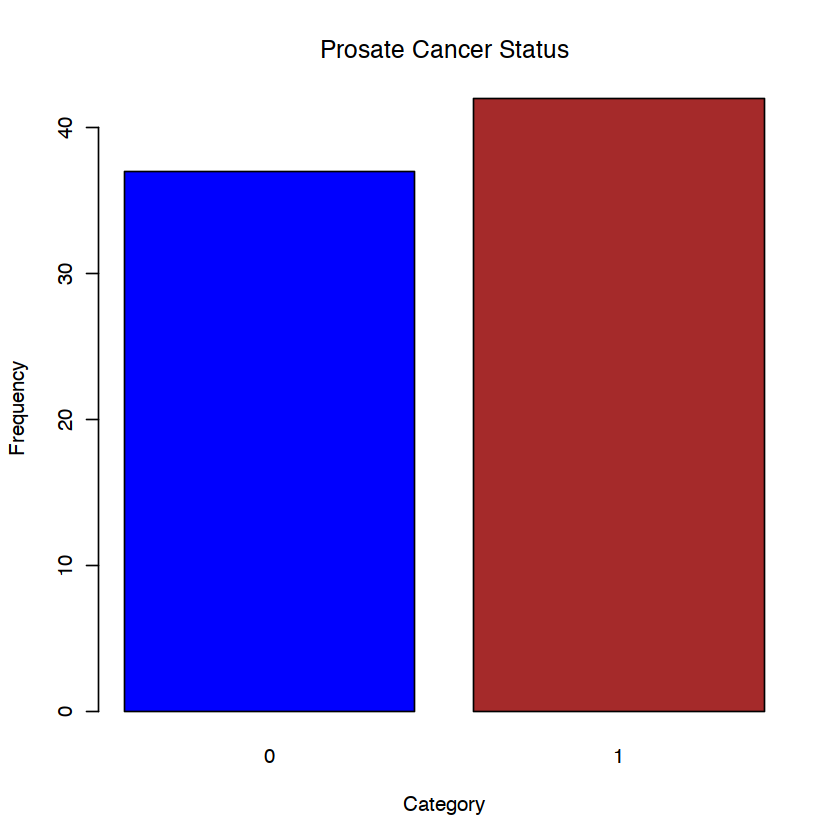
\includegraphics[width=480pt,height=420pt]{./graphics/q21.png}
				\caption{Barchart distribution of response variable}
				\label{fig:01}
		\end{figure}
		
		Prostate Cancer Microarray Gene Expression  dataset has a size of 79 observations  and 500  variables in which  0 indicates people not suffering from prostate cancer while 1 represent people with prostate cancer . And from Figure \ref{fig:01},  it means that 37 out of 79 are not suffering while 42 out of 79 are suffering from prostate cancer.  In percentage terms,  46.84 \% are not suffering while 53.16 \% are suffering prostate cancer.
		\item[(3)]  Comment on the shape of this dataset in terms of the sample size and the dimensionality of the input space.\\
		From the observation of the dataset $n= 79$ and $p=500,$ which implies  $p>>n$ therefore the dataset is ultra high dimensional.	
			\item[(4)] Comment succinctly from the statistical perspective on the type of data in the input space.  It is absolutely crucial here to provide as many details as possible including distributional aspects via boxplots and others on randomly selected subsets of variables.
			\begin{figure}[!h]
				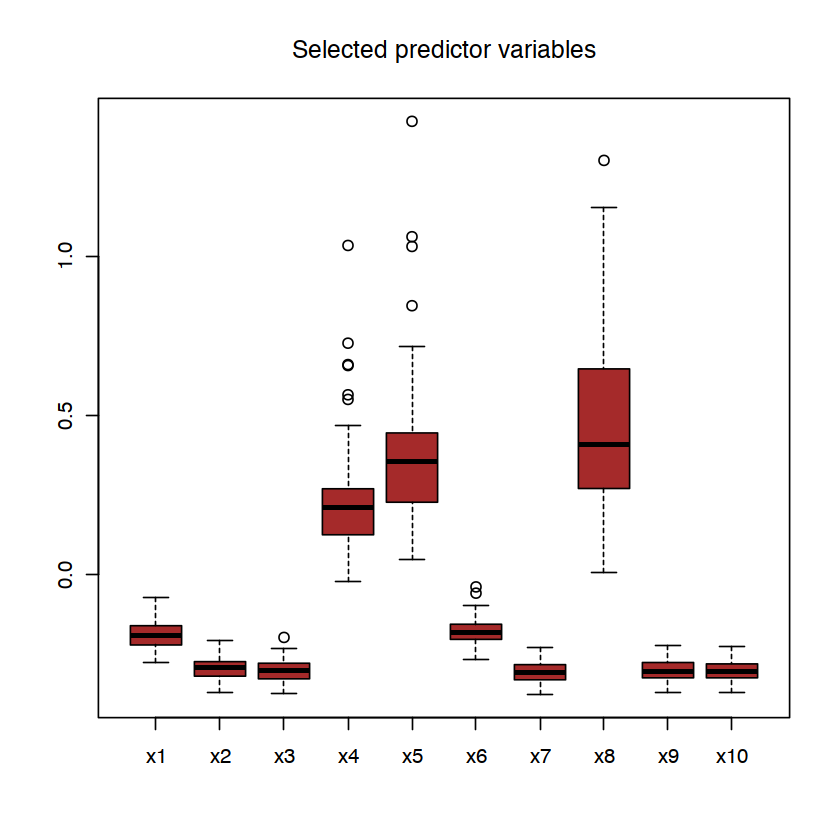
\includegraphics[width=420pt,height=350pt]{./graphics/q24.png}
				\caption{A distribution  bloxplot of selected independent variables}
				\label{fig:02}
		\end{figure}
		
%			\begin{figure}[!h]
%				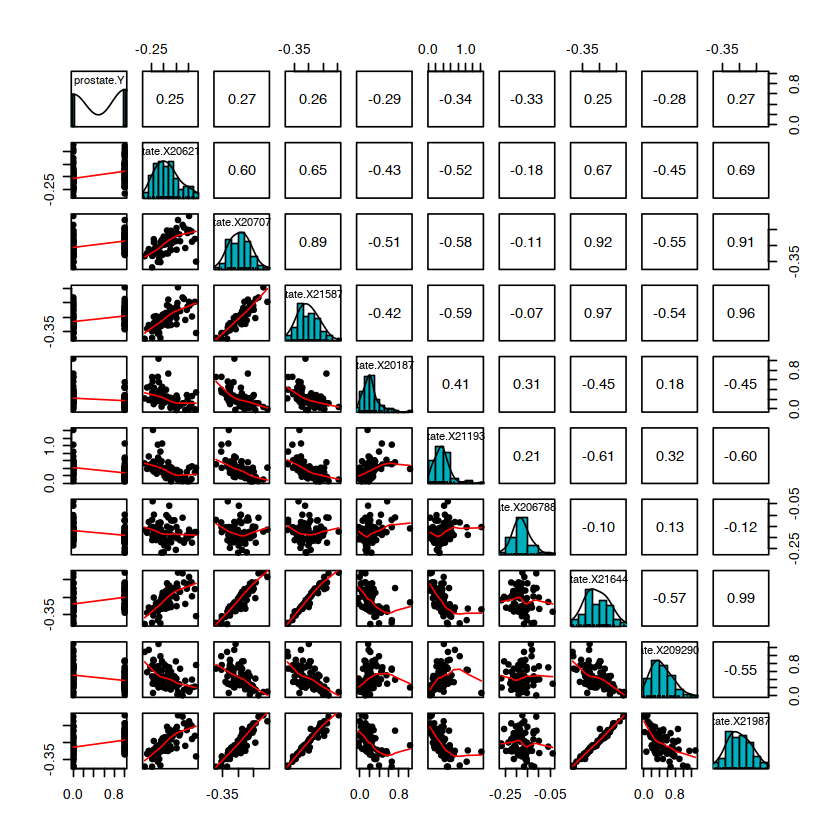
\includegraphics[width=420pt,height=350pt]{./graphics/q24b.png}
%				\caption{A distribution matrix of selected independent variables}
%				\label{fig:03}
%		\end{figure}
			- From the figure \ref{fig:03}, we can clearly observe that the median line from selected variables $x_2,x_3,x_7,x_9,x_10$ are almost equal, hence being symmetrically distributed (Normally distributed).\\
			- Expect variable $x_3,x_4,x_5,x_6,x_8$, we can see that there is no outliers in other selected variables.\\
			- Apart from $x_4,x_5,x_8$,  all other remaining variables are in the same range.
\end{enumerate}

\section*{Exercise 3}
Given 
\begin{center}
$
	X  = 
	\begin{bmatrix}
		1 & -2 \\
		-2 & 1\\
		4 & 1
	\end{bmatrix} \quad 
	Y = \begin{bmatrix}
			-5 \\
			4\\
			-3
	\end{bmatrix}
	$
\end{center}
\begin{enumerate}
	\item[(1)] Compute $X^{\text{T}}X$
			\begin{align*}
						X^{\text{T}}X &=  
						\begin{bmatrix}
							1 & -2 & 4 \\
							-2 & 1 & 1
						\end{bmatrix}
					 	\begin{bmatrix}
								1 & -2 \\
								-2 & 1\\
							4 & 1
						\end{bmatrix}\\
						&=  \begin{bmatrix}
								21 & 0\\
								0 & 6
						\end{bmatrix}
			\end{align*}
		\item[(2)] Comment on the shape of $X^{\text{T}}X $
				\begin{itemize}
						\item $X^{\text{T}}X $ is a diagonal matrix.
				\end{itemize}
		\item[(3)] Find  $(X^{\text{T}}X)^{-1} $ in the most straightforward way
					\begin{align*}
							(X^{\text{T}}X)^{-1}  &=  \text{Diag}(u) \quad  \text{where }  u= \begin{pmatrix}
						\frac{1}{21} , \frac{1}{6}		
							\end{pmatrix}^{\text{T}}							 
					\end{align*}
		\item[(4)] Compute $\hat{\theta} =( X^{\text{T}}X)^{-1} X^{\text{T}}Y $ 
					\begin{align*}
							X^{\text{T}}Y  &=  \begin{bmatrix}
							1 & -2 & 4 \\
							-2 & 1 & 1
						\end{bmatrix} 
						\begin{bmatrix}
								-5 \\
								4\\
								-3
						\end{bmatrix} =   \begin{bmatrix}
			-25\\
			11
	\end{bmatrix}
					\end{align*}
					
					\begin{align*}
						( X^{\text{T}}X)^{-1}  &=   \begin{bmatrix}
								\frac{1}{21} & 0\\
								0 & \frac{1}{6}
						\end{bmatrix}
					\end{align*}
			\begin{align*}
					( X^{\text{T}}X)^{-1} X^{\text{T}}Y  &=   \begin{bmatrix}
								\frac{1}{21} & 0\\
								0 & \frac{1}{6}
						\end{bmatrix}    \begin{bmatrix}
			-25\\
			11
	\end{bmatrix} \\
	  &=  \begin{bmatrix}
			\frac{-25}{21}\\
			\frac{11}{6}
	\end{bmatrix}
			\end{align*}
		\item[(5)] Compute the vector $\hat{Y} $ of estimated responses
		
		\begin{align*}
			\hat{Y}  &=  X\hat{\Theta}\\
				&= \begin{bmatrix}
								1 & -2 \\
								-2 & 1\\
							4 & 1
						\end{bmatrix}  \begin{bmatrix}
			\frac{-25}{21}\\
			\frac{11}{6}
	\end{bmatrix}\\
	 &=  \begin{bmatrix}
			\frac{-34}{7}\\
			\frac{59}{14}\\
			\frac{-41}{14}
	\end{bmatrix}
		\end{align*}
	\item[(6)] Compute the vector $e $ of the residual values
	\begin{align*}
			e &= = Y - \hat{Y} \\
			&=   \begin{bmatrix}
			-5 \\
			4\\
			-3
	\end{bmatrix} - \begin{bmatrix}
			\frac{-34}{7}\\
			\frac{59}{14}\\
			\frac{-41}{14}
	\end{bmatrix}
	&=  \begin{bmatrix}
			\frac{-1}{7}\\
			\frac{-3}{14}\\
			\frac{-1}{14}
	\end{bmatrix}
	\end{align*}
	\item[(7)] Find the value of $\text{SSE}(\hat{\theta})$
		\begin{align*}
					\text{SSE}(\hat{\theta}) &=  \sum(Y - \hat{Y})^2\\
					&=  \frac{1}{49} + \frac{9}{196} + \frac{1}{196} \\
					&= \frac{1}{14}
		\end{align*}
	\item[(8)]  Find the estimated $\hat{\sigma^2}$
		\begin{align*}
			\hat{\sigma^2} &=  \frac{\text{SSE}(\hat{\theta})}{n -2} \\
			\text{Since $n = 3$ \quad }   \\
			\frac{\text{SSE}(\hat{\theta})}{n -2} &= \frac{1}{14}
		\end{align*}
	\item[(9)] Find and write down Variance$(\hat{\sigma^2})$
	\begin{align*}
			\text{Variance}(\hat{\sigma^2}) &= \hat{\sigma^2} (X^{\text{T}}X)^{-1} \\
			&=  \frac{1}{14} \begin{bmatrix}
								\frac{1}{21} & 0\\
								0 & \frac{1}{6}
						\end{bmatrix}\\
			&= \begin{bmatrix}
								\frac{1}{294} & 0\\
								0 & \frac{1}{84}
						\end{bmatrix}
	\end{align*}
	\item[(10)] Write the matrix $(X^{\text{T}}X)$ in a function of the identity matrix when the data matrix is given by:
		\begin{align*}
				X & = \begin{bmatrix}
							1 & -2\\
							2 & 1
				\end{bmatrix}\\
				X^{\text{T}}X &=  \begin{bmatrix}
							1 & 2\\
							-2 & 1
				\end{bmatrix}  \begin{bmatrix}
							1 & -2\\
							2 & 1
				\end{bmatrix}\\
				&=  \begin{bmatrix}
							5 & 0\\
							0 & 5
				\end{bmatrix}
		\end{align*}
	In the form of an identity matrix 
	\begin{align*}
			X^{\text{T}}X 	&=  5 \begin{bmatrix}
							1 & 0\\
							0 & 1
				\end{bmatrix}
	\end{align*}
\end{enumerate}
\pagebreak
\section*{Exercise 4}
\begin{enumerate}
	\item[(1)] Generate an upper triangular pairwise scatterplot for this data, and comment based onthe scatterplots regarding which of the explanatory variables aremore strongly related tothe response. Can you tell from the plot the strongest of all the predictor variables?\\
			\begin{figure}[!h]
				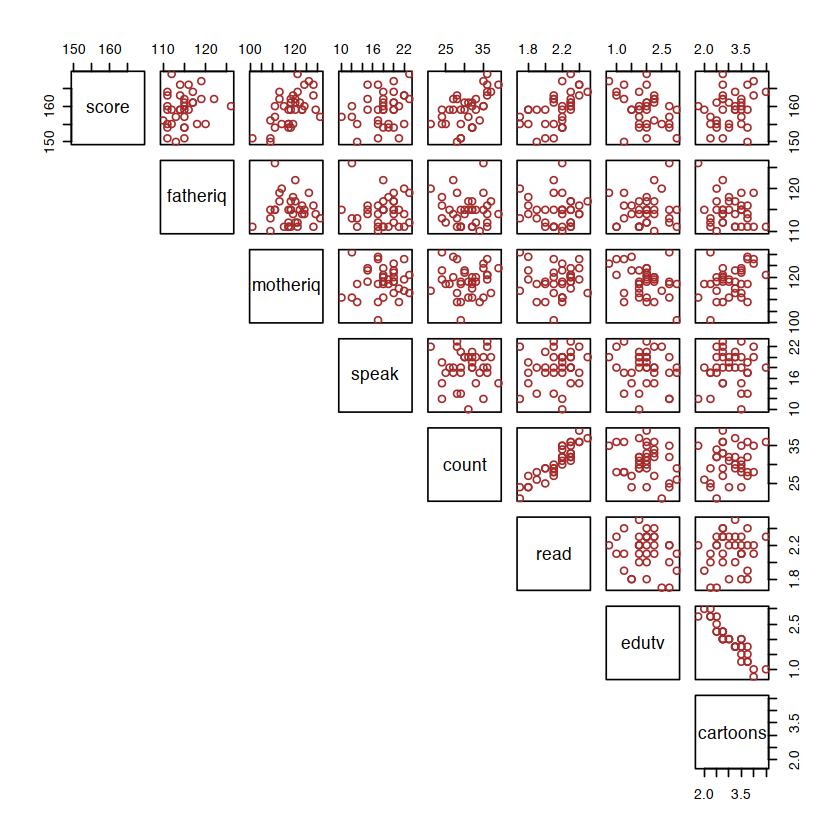
\includegraphics[width=520pt,height=450pt]{./graphics/q41.png}
				\caption{Correlation plot of independent variables to score}
				\label{fig:03}
		\end{figure}
\\From the scatterplots  in \ref{fig:03},  3 variables are linearly correlated to score which are \textbf{motheriq, count} and \textbf{read} amongst which motheriq has the strongest linear correlation to the response score.
	\item[(2)]  Generate the correlation matrix for this data (please do not include the p-values in thematrix for now). Which variable does the correlation matrix appear to indicate as the strongest?\\
			% Please add the following required packages to your document preamble:
% \usepackage[table,xcdraw]{xcolor}
% If you use beamer only pass "xcolor=table" option, i.e. \documentclass[xcolor=table]{beamer}
% Please add the following required packages to your document preamble:
% \usepackage[table,xcdraw]{xcolor}
% If you use beamer only pass "xcolor=table" option, i.e. \documentclass[xcolor=table]{beamer}
\begin{table}[!h]
\begin{tabular}{cllllllll}
\textbf{} & \multicolumn{1}{c}{\textbf{score}} & \multicolumn{1}{c}{\textbf{fatheriq}} & \multicolumn{1}{c}{\textbf{motheriq}} & \multicolumn{1}{c}{\textbf{speak}} & \multicolumn{1}{c}{\textbf{count}} & \multicolumn{1}{c}{\textbf{read}} & \multicolumn{1}{c}{\textbf{edutv}} & \multicolumn{1}{c}{\textbf{cartoons}} \\
\textbf{score} & 1.00 & 0.19 & {\color[HTML]{FD6864} 0.57} & 0.27 & 0.54 & 0.53 & -0.37 & 0.25 \\
\textbf{fatheriq} & 0.19 & 1.00 & -0.02 & -0.03 & -0.08 & -0.07 & 0.12 & -0.25 \\
\textbf{motheriq} & {\color[HTML]{FE0000} 0.57} & -0.02 & 1.00 & 0.07 & 0.02 & -0.04 & -0.33 & 0.34 \\
\textbf{speak} & 0.27 & -0.03 & 0.07 & 1.00 & 0.06 & 0.19 & -0.15 & 0.11 \\
\textbf{count} & 0.54 & -0.08 & 0.02 & 0.06 & 1.00 & 0.91 & -0.22 & 0.15 \\
\textbf{read} & 0.53 & -0.07 & -0.04 & 0.19 & 0.91 & 1.00 & -0.17 & 0.13 \\
\textbf{edutv} & -0.37 & 0.12 & -0.33 & -0.15 & -0.22 & -0.17 & 1.00 & -0.92 \\
\textbf{cartoons} & 0.25 & -0.25 & 0.34 & 0.11 & 0.15 & 0.13 & -0.92 & 1.0
\end{tabular}
\caption{Correlation matrix}
\label{tab:1}
\end{table}
From table \ref{tab:1} above, the correlation matrix clearly indicates the predictor variable \textbf{motheriq} has  the strongest linear correlation with score (the response variable).
\item[(3)] Plot a histogram of the response variable and also perform a test of normality on it.\\
			\begin{figure}[!h]
				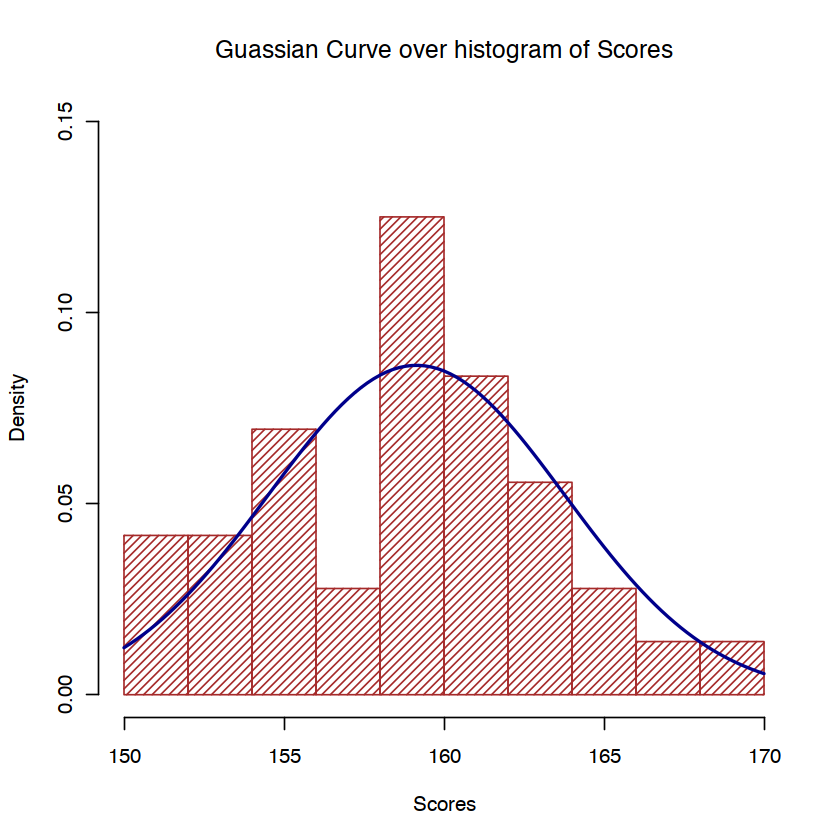
\includegraphics[width=370pt,height=310pt]{./graphics/q43b.png}
				\caption{histogram of response variable score}
				\label{fig:04}
		\end{figure}
		
\textbf{Formal Test of Normality}\\
$\mathbb{H}_0 $ The response variable \textbf{score} is normally distributed while  $\mathbb{H}_1$  \textbf{score} is not normally distributed.
\begin{verbatim}
			Shapiro-Wilk normality test
			
	data:  gifted$score
	W = 0.98051, p-value = 0.7625
\end{verbatim}
From Figure \ref{fig:04} above and the Shapiro-Wilk Normality test where the p-value = 0.7625 which is greater than the Significance Level $\alpha = 0.05$,  we fail to reject $\mathbb{H}_0$ and conclude that the response variable is normally distributed.
\item[(4)] Perform a simple linear regression (SLR) model fitting featuring the response and the variable you singled out as the most important.\\
\begin{verbatim}
		SLR <-  lm(score  motheriq, data = gifted)
\end{verbatim}
Simple Linear Regression Model: 
\begin{align*}
		\hat{score} = 111.0930 + 0.4066 \times  \text{motheriq}
\end{align*}
\item[(5)] Generate the 4 residual analysis plots and comment on the suitability of your built model.Are there observations that might have badly influenced the estimation of your parameters?
			\begin{figure}[!h]
				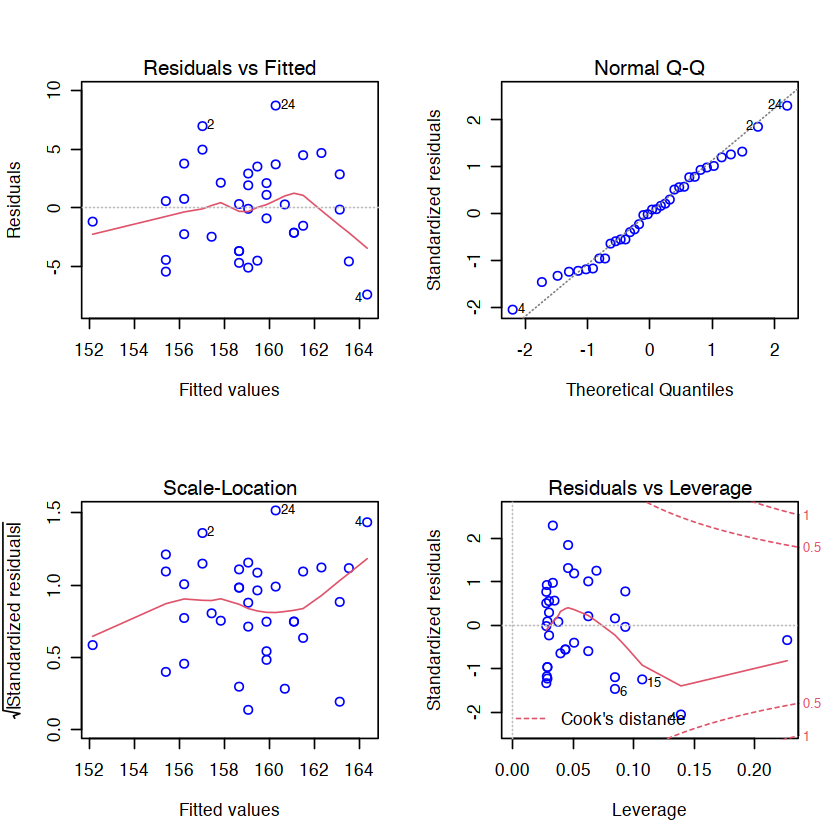
\includegraphics[width=460pt,height=340pt]{./graphics/q45.png}
				\caption{SLR Residual Plot}
				\label{fig:05}
		\end{figure}
We can infer the following properties of the model from the residual plot in Figure \ref{fig:05}. The plot of Residuals vs Fitted indicates the linearity assumption is met.  Normal Q-Q plot shows the we have normality.  From Scale-Location plot the model has homoskedacity and Residuals vs Leverage shows that we have outliers.
\item[(6)] Let’s assume for a little while that you are to use the above SLR model. Then give an interpretation of your estimated slope in layman’s term.\\
\begin{verbatim}
Coefficients:
            Estimate Std. Error t value Pr(>|t|)    
(Intercept) 111.0930    11.8567   9.370 6.02e-11 ***
motheriq      0.4066     0.1002   4.058 0.000274 ***
---
Signif. codes:  0 ‘***’ 0.001 ‘**’ 0.01 ‘*’ 0.05 ‘.’ 0.1 ‘ ’ 1

Residual standard error: 3.856 on 34 degrees of freedom
Multiple R-squared:  0.3263,	Adjusted R-squared:  0.3065 
F-statistic: 16.47 on 1 and 34 DF,  p-value: 0.000274
\end{verbatim}
From the above summary,  a unit increase in \textbf{motheriq} will increase  \textbf{score} by 0.4066.
\item[(7)] Generate both confidence bands and the prediction bands for this model and provide intelligent comments on what you get.\\
			\begin{figure}[!h]
				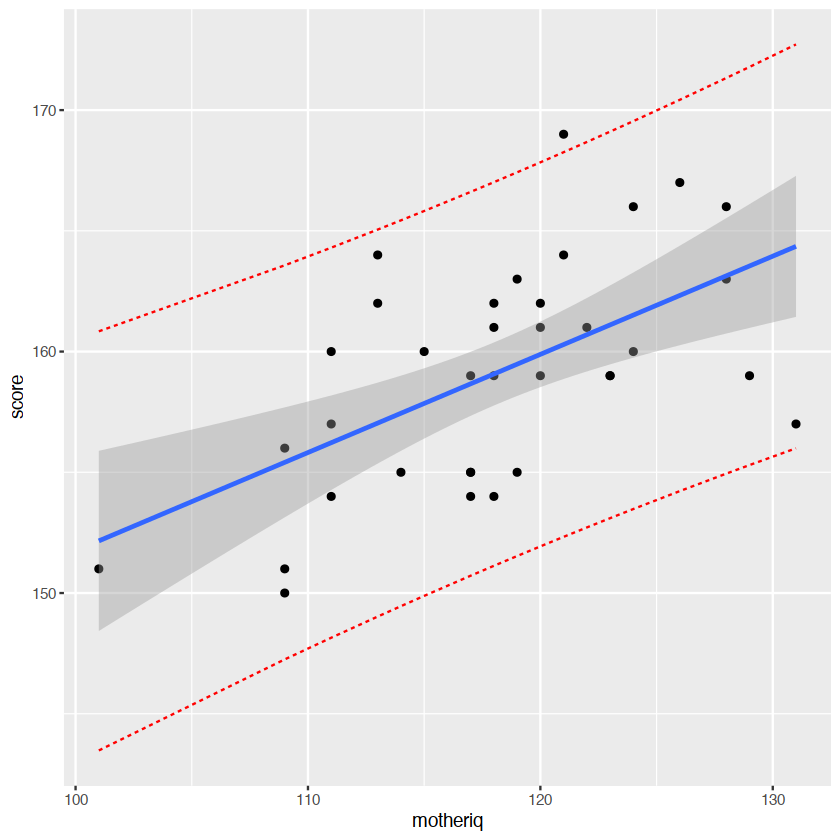
\includegraphics[width=420pt,height=310pt]{./graphics/q47.png}
				\caption{SLR Prediction Band}
				\label{fig:06}
		\end{figure}
		
	The Prediction interval (PI) in Figure \ref{fig:06} is an estimate of an interval in which a future observation will fall,  with a certain confidence level,  given the observations that were already observed. 
		\begin{figure}[!h]
				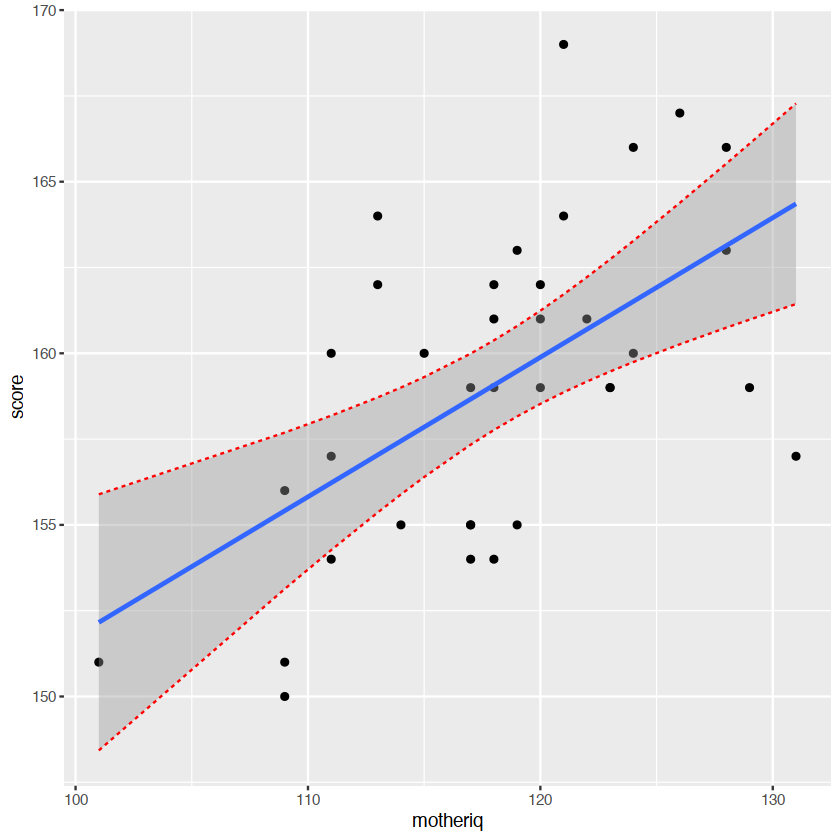
\includegraphics[width=420pt,height=320pt]{./graphics/q47b.png}
				\caption{SLR Confidence Band}
				\label{fig:07}
		\end{figure}
		From Figure \ref{fig:07}, the confidence interval (lower line and upper red lines) signifies the range in which the true population parameter lies at a 95\% level of confidence.  This functionally means is that we're 95\% confident that the true regression line lies somewhere in that gray zone.
	\item[(8)] Build a multiple linear regression (MLR) model for this data comprising of all the provided explanatory variables.\\
	\begin{verbatim}
		Coefficients:
            Estimate Std. Error t value Pr(>|t|)    
(Intercept) 75.50849   24.02618   3.143  0.00393 ** 
motheriq     0.40007    0.07291   5.488 7.33e-06 ***
fatheriq     0.25249    0.13756   1.835  0.07707 .  
speak        0.18764    0.14767   1.271  0.21429    
count        0.20649    0.26631   0.775  0.44462    
read         7.54405    5.58640   1.350  0.18769    
edutv       -4.20244    2.24503  -1.872  0.07170 .  
cartoons    -3.33899    2.01808  -1.655  0.10919    
---
Signif. codes:  0 ‘***’ 0.001 ‘**’ 0.01 ‘*’ 0.05 ‘.’ 0.1 ‘ ’ 1

Residual standard error: 2.591 on 28 degrees of freedom
Multiple R-squared:  0.7496,	Adjusted R-squared:  0.687 
F-statistic: 11.97 on 7 and 28 DF,  p-value: 5.803e-07
	\end{verbatim}
	
	From observing the $\text{Pr}(>|t|) $ values of the predictor variables, we can draw a conclusion that \textbf{motheriq} has the strongest factor of variation (explanatory power) in the response variable as compared to the others because is has a p-value significantly lower than the Significance Level $\alpha = 0.05$.
\end{enumerate}
\end{document}